% --------------------------------------------------
%  Week 1 – Mathematical Modeling of Disease Spread
%  Version 1 (10 June 2025)
%  Figures resized so they sit correctly on 16:9 slides
% --------------------------------------------------
\documentclass[14pt,aspectratio=169]{beamer}
\usetheme{Madrid}

% --------------------------------------------------
%          Packages
% --------------------------------------------------
\usepackage{amsmath,amsfonts,siunitx}
\usepackage{graphicx}
\usepackage{hyperref}
\usepackage[absolute,overlay]{textpos}
\definecolor{VUblue}{HTML}{002F6C}
\setbeamercolor{alerted text}{fg=VUblue}
\setbeamercolor{structure}{fg=VUblue}
% Graphics path & defaults – every figure is at most 45 % of text height
\graphicspath{{Figures/}}
\setkeys{Gin}{height=0.45\textheight,keepaspectratio}

% Textpos grid = centimetres (easier positioning)
\setlength{\TPHorizModule}{1cm}
\setlength{\TPVertModule}{1cm}

% --------------------------------------------------
%          Macros
% --------------------------------------------------
\newcommand{\dd}{\,\mathrm{d}}
\newcommand{\RR}{\mathcal{R}_0}

% --------------------------------------------------
%          Metadata
% --------------------------------------------------
\title[Modeling Disease Spread]{Key Ideas from Week 1\\Mathematical Modeling of Disease Spread}
\author{J.~Graham \and T.~Molenaar \and E.~Terjyan}
% break institute into two lines and reduce font size
\setbeamerfont{institute}{size=\footnotesize}
\institute[VU Amsterdam]{%
  Vrije University\
  of Amsterdam \\
  Dynamical Systems Project
}\date{10 June 2025}

% --------------------------------------------------
\begin{document}

% --------------------------------------------------
\begin{frame}[plain]
  \titlepage
\end{frame}

% --------------------------------------------------
\begin{frame}{Motivation \& Questions}
  \begin{itemize}
    \item \textbf{Public‑health planning:} How many will be infected? When should we intervene?
    \item \textbf{Today’s focus = core mechanisms}
      \begin{itemize}
        \item Infection only (\alert{SI})
        \item Recovery only (\alert{IR})
        \item Infection \& recovery combined (\alert{SIS})
      \end{itemize}
    \item Guiding question: \alert{What determines if an outbreak continues transmission?}
  \end{itemize}
\end{frame}
% --------------------------------------------------
% \begin{frame}{Motivation \& Questions}
%   \begin{itemize}
%     \item \textbf{Public‑health planning:} How many will be infected? When should we intervene?
%     \item \textbf{Today’s focus = core mechanisms}
%       \begin{itemize}
%         \item Infection only (\alert{SI})
%         \item Recovery only (\alert{IR})
%         \item Infection \& recovery combined (\alert{SIS})
%       \end{itemize}
%     \item Guiding question: \alert{What determines if an outbreak continues transmission?}
%   \end{itemize}
% \end{frame}

% --------------------------------------------------
\begin{frame}{Basic notation (closed population $N$)}
  \begin{block}{State variables (total numbers)}
    \begin{description}
      \item[$S(t)$] Susceptible individuals
      \item[$I(t)$] Infectious individuals
    \end{description}
    Always $S+I=N$ (no births, no deaths).
  \end{block}
  \vspace{0.5em}
  \begin{block}{Parameters}
    \begin{itemize}
      \item Contact rate $c$ (contacts·day$^{-1}$)
      \item Per‑contact transmission probability $p$
      \item Recovery rate $\gamma$ (day$^{-1}$)
    \end{itemize}
    \vspace{0.3em}
    \alert{$\beta = c\,p$}\hfill(effective contact rate, day$^{-1}$)
  \end{block}
\end{frame}

% --------------------------------------------------
%   3. SI model
% --------------------------------------------------
\begin{frame}{The SI model: infection only}
  \[
    \frac{\dd I}{\dd t}=\beta I\frac{S}{N}
    \quad\Longrightarrow\quad
    \frac{\dd I}{\dd t}=\beta I\!\left(1-\frac{I}{N}\right)
  \]
  \begin{itemize}
    \item Logistic growth $\Rightarrow$ analytic solution
    \item \textbf{Outcome:} Everyone is eventually infected ($I\to N$)
  \end{itemize}
  \centering
  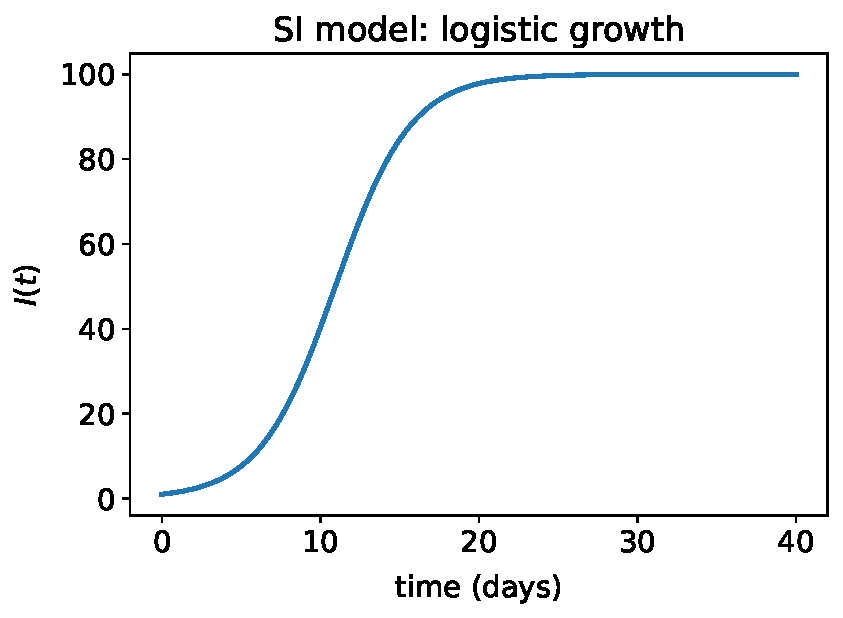
\includegraphics{LogisticIllustration.pdf}
  \begin{textblock*}{\textwidth}(0cm,8.45cm)
    {\scriptsize Axes: \emph{time $t$} (days) vs. \emph{infectious individuals $I(t)$}}
  \end{textblock*}
\end{frame}

% --------------------------------------------------
%   4. IR model
% --------------------------------------------------
\begin{frame}{The IR model: recovery only}
  \[
    \frac{\dd I}{\dd t}=-\gamma I
    \quad\Longrightarrow\quad
    I(t)=I_0\,e^{-\gamma t}
  \]
  \begin{itemize}
    \item Mean infectious period $=1/\gamma$
    \item \textbf{Outcome:} Exponential decay to zero
  \end{itemize}
  \centering
  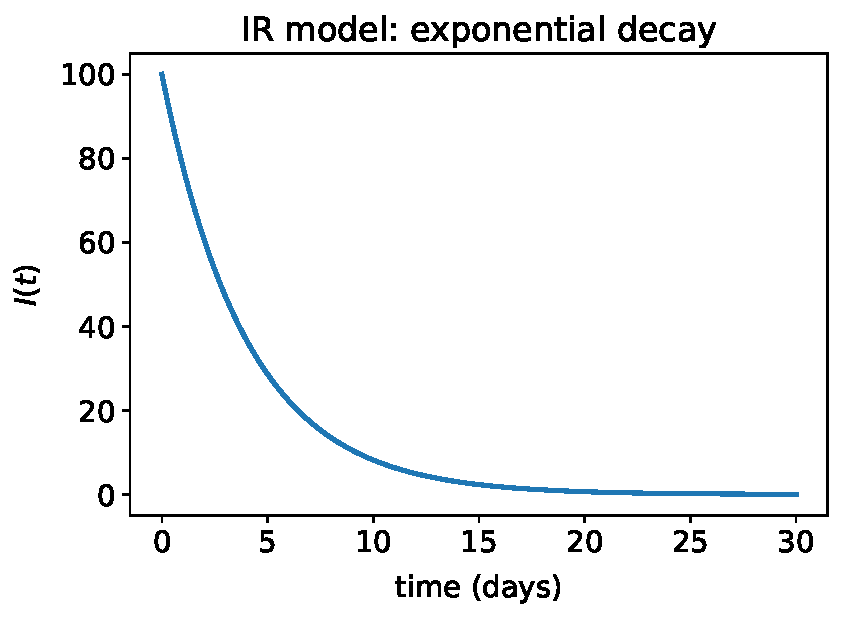
\includegraphics{DecayIllustration.pdf}
  \begin{textblock*}{\textwidth}(0cm,8.4cm)
    {\scriptsize Axes: \emph{time $t$} (days) vs. \emph{infectious individuals $I(t)$}}
  \end{textblock*}
\end{frame}

% --------------------------------------------------
%   5. SIS model equations
% --------------------------------------------------
\begin{frame}{SIS model = SI + IR}
  \[
    \frac{\dd I}{\dd t}=\beta I\frac{S}{N}-\gamma I
    \quad\Longrightarrow\quad
    \underbrace{\frac{\dd i}{\dd \tau}=\RR\,i(1-i)-i}_{\textstyle i=I/N,\;\tau=\gamma t}
  \]
  \begin{block}{Basic reproduction number}
    \[
      \RR = \frac{\beta}{\gamma}\quad=\text{expected secondary cases per primary case}
    \]
  \end{block}
  \begin{itemize}
    \item Disease‑free equilibrium $(i=0)$
    \item Endemic equilibrium $i^*=1-\tfrac1{\RR}$ if $\RR>1$
  \end{itemize}
\end{frame}

% --------------------------------------------------
%   6. Time‑series demo
% --------------------------------------------------
\begin{frame}{Numerical example ($\beta=0.42$, $\gamma=0.25$)}
  \centering
  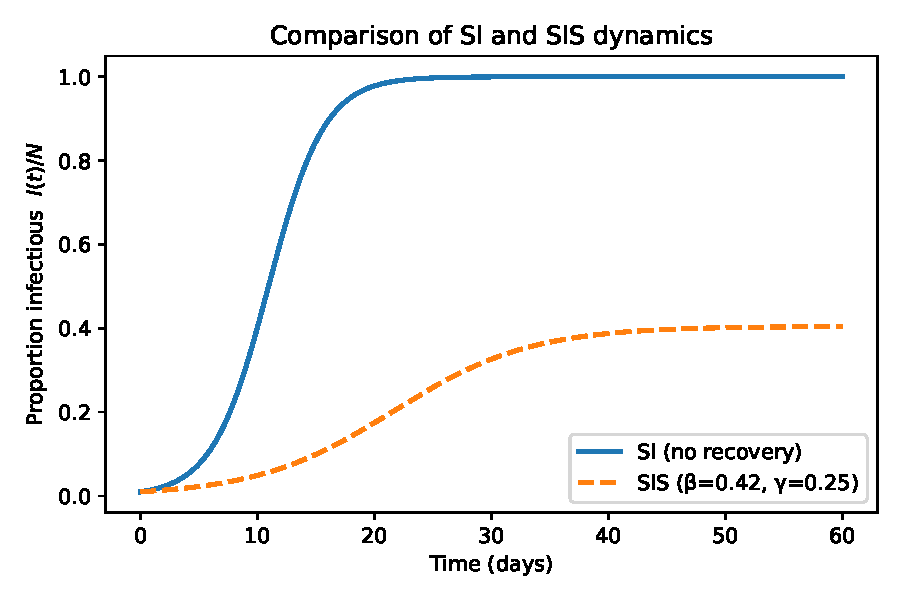
\includegraphics{Timeseries.pdf}
  \begin{textblock*}{\textwidth}(0cm,6cm)
    {\scriptsize Axes: \emph{time (days)} vs. \emph{infectious proportion $I/N$}}
  \end{textblock*}
  \vspace{-0.3em}
  \begin{itemize}
    \item $\RR\approx1.68>1$ $\Rightarrow$ outbreak peaks then settles at an endemic level.
  \end{itemize}
\end{frame}

% --------------------------------------------------
%   7. Key take‑aways
% --------------------------------------------------
\begin{frame}{Key messages}
  \begin{enumerate}
    \item Infection pressure $\beta$ alone drives unlimited growth (SI).
    \item Recovery $\gamma$ alone drives exponential die‑out (IR).
    \item Together they form the \alert{threshold} $\RR=\beta/\gamma$ (SIS):
      \[
        \RR>1\;\Rightarrow\;\textbf{sustained transmission},\quad
        \RR \leq 1\;\Rightarrow\;\textbf{fade‑out}
      \]
  \end{enumerate}
\end{frame}

% --------------------------------------------------
%   8. Wrap‑up
% --------------------------------------------------
\begin{frame}{Conclusions \& Outlook}
  \begin{itemize}
    \item Modeling reveals which knobs matter: lowering $\beta$ or raising $\gamma$ cuts $\RR$.
    \item Next step (SIR) adds immunity: What if recovered individuals \emph{stay} immune?
    \item All code and \LaTeX\ at:\  \href{https://github.com/ernestterjyan/mathematical_model_DS}{github.com/ernestterjyan/mathematical\_model\_DS}
  \end{itemize}
  \vfill
  \centering{\Large Thank you!}
\end{frame}

% --------------------------------------------------
% References
\begin{frame}[allowframebreaks]{References}
  \begin{thebibliography}{9}
    \bibitem{Kermack1927} W.~O.~Kermack and A.~G.~McKendrick,
      "A Contribution to the Mathematical Theory of Epidemics," 
      \textit{Proc. Roy. Soc. A}, vol.~115, pp.~700--721, 1927.
    \bibitem{Greer2018} M.~L.~Greer and D.~R.~Livesay,
      \textit{An Introduction to Mathematical Epidemiology}, Springer, 2018.
    \bibitem{Mossong2008} J.~Mossong \textit{et al.},
      "Social Contacts and Mixing Patterns Relevant to the Spread of Infectious Diseases," 
      \textit{PLoS Med.}, vol.~5, no.~3, e74, 2008.
    \bibitem{cdcYellowBook2024} Centers for Disease Control and Prevention,
      "Influenza – Travellers’ Health, CDC Yellow Book 2024," 2024.
      [Online]. Available: \url{https://wwwnc.cdc.gov/travel/yellowbook/2024/infections-diseases/influenza}
      (accessed Jun.~6, 2025).
  \end{thebibliography}
\end{frame}
\end{document}
